\documentclass[hyperref={pdfpagelabels=false}]{beamer}
\usepackage[utf8]{inputenc}
% By  using hyperref={pdfpagelabels=false} you get rid off:
% Package hyperref Warning: Option `pdfpagelabels' is turned off
% (hyperref)                because \thepage is undefined. 
% Hyperref stopped early 
%

\usepackage{lmodern}
% Using lmondern and you get rid off this:
% LaTeX Font Warning: Font shape `OT1/cmss/m/n' in size <4> not available
% (Font)              size <5> substituted on input line 22.
% LaTeX Font Warning: Size substitutions with differences
% (Font)              up to 1.0pt have occurred.
%

% If \titel{$B!D(B} \author{$B!D(B} come after \begin{document} 
% you get the following warnig:
% Package hyperref Warning: Option `pdfauthor' has already been used,
% (hyperref) ... 
% So it is here before \begin{document}

\usetheme{AnnArbor}
\usecolortheme{beaver}
\title{Artificial financial market }   
\author{Fabián Romero} 
\date{Jingyuan Ding } 
% additional usepackage{beamerthemeshadow} is used

%\usepackage{beamerthemeshadow}

\begin{document}

\begin{frame}
\titlepage
\end{frame} 

\begin{frame}
\frametitle{Table of contents}
\tableofcontents
\end{frame}
 
\section{Introducción} 
\begin{frame}
\frametitle{Referencia} 
Jingyuan Ding (2011). Cellular Automata based Artificial Financial Market, Cellular Automata - Simplicity
Behind Complexity, Dr. Alejandro Salcido (Ed.), ISBN: 978-953-307-230-2, InTech, Available from:

\url{http://www.intechopen.com/books/cellular-automata-simplicity-behind-complexity/cellular-automata-based-artificial-financial-market}

\end{frame}

\subsection{Conceptos básicos}
\begin{frame}
\frametitle{Conceptos básicos} 

\begin{itemize}

\item Teoría del mercado de capitales
\begin{itemize}
\item Rational investor hypothesis
\item Efficient markets hypothesis(EMH)
\item Random walk
\end{itemize}
\item Simulación
\begin{itemize}
\item multi-agent system (MAS)
\item cellular automata (CA)\\
 Santa Fe artificial stock market(SF-ASM)\\
 Es mas ``eficiente'' que los mercados de capital reales
\end{itemize}
\end{itemize}
\end{frame}


\section{Mercado de capitales como sistema complejo} 
\subsection{Sistemas complejos}
\begin{frame}
\frametitle{Mercado de capitales como sistema complejo}
\begin{itemize}
\item Las teorias descritas no representan el comportamiento ni la psicología de las inversiones
\item Gran cantidad de individuos con metas autónomas
\item interacción local - efectos globales
\end{itemize} 
\end{frame}

\begin{frame}
\frametitle{Santa Fe Institute artificial stock market}
En cada momento $t$ el agente $i$ tiene algunas acciones del mercado $h_i(t)$ y tiene una parte de dinero resguardado $M_i(t)$, por lo que los bienes del agente $i$ son:

$$ w_i(t)= M_i(t)+h_i(t)*p(t)$$

La información se propaga en el mercado, al mismo tiempo y será manejado por los agentes inmediatamente. Simplificación excesiva de la información y haciendo caso omiso de la interacción local.
\end{frame}

\begin{frame}
\frametitle{El modelo clásico basado en autómatas celulares}
Es necesario describir la interacción entre de los individuos, si queremos construir un modelo para la difusión de la información no pública. Los autómatas celulares son superiores en este aspecto.

En este modelo, el mercado de valores es considerado como un autómata celular. Y los inversionistas se consideran como las células en el espacio 2D. Se usa la vecindad de Moore


Comportamiento de rebaño en el mercado de capitales. En el modelo, una célula tiene sólo tres estados (actitud): comprar, mantener y vender. En el paso t, el estado de la celda sería decidida por los estados de los vecinos en el paso t-1.

\begin{itemize}
\item d-dimensional
\item HPP Lattice Gas Automata(Hardy et al.,1973)
\item FHP Lattice Gas Automata (Frisch et al., 1986)
\item latice hexagonal
\end{itemize} 

\end{frame}

\subsection{The Emergence-Artificial Financial Market Framework (E-AFM)}
\begin{frame}
\frametitle{The Emergence-Artificial Financial Market Framework (E-AFM)}
\begin{enumerate}
\item Exponente de Hurst  (análisis de series de tiempo financieras), esoecufucamente la ``memoria a largo plazo'' y Analisis de Rango Ajustado (Rescaled Range Analysis)
\item 
Rango ajustado $lim_{N \to \infty}  E(R_n/S_n)=(aN)^H$
con $ log(E(R_n/S_N)) = H log(N) + log(a)$

$H$ es el exponente de Hurst, que se puede estimar por el método de ``least square''
y el coeficiente de ``clustering'' $\gamma_v$ de una celda $v$ es definida como:

$$ \gamma_v = \frac{E(\Gamma_v)}{\binom{k_v}{2}} $$


\end{enumerate}
\end{frame}

\begin{frame}
\frametitle{Análisis dinámico}
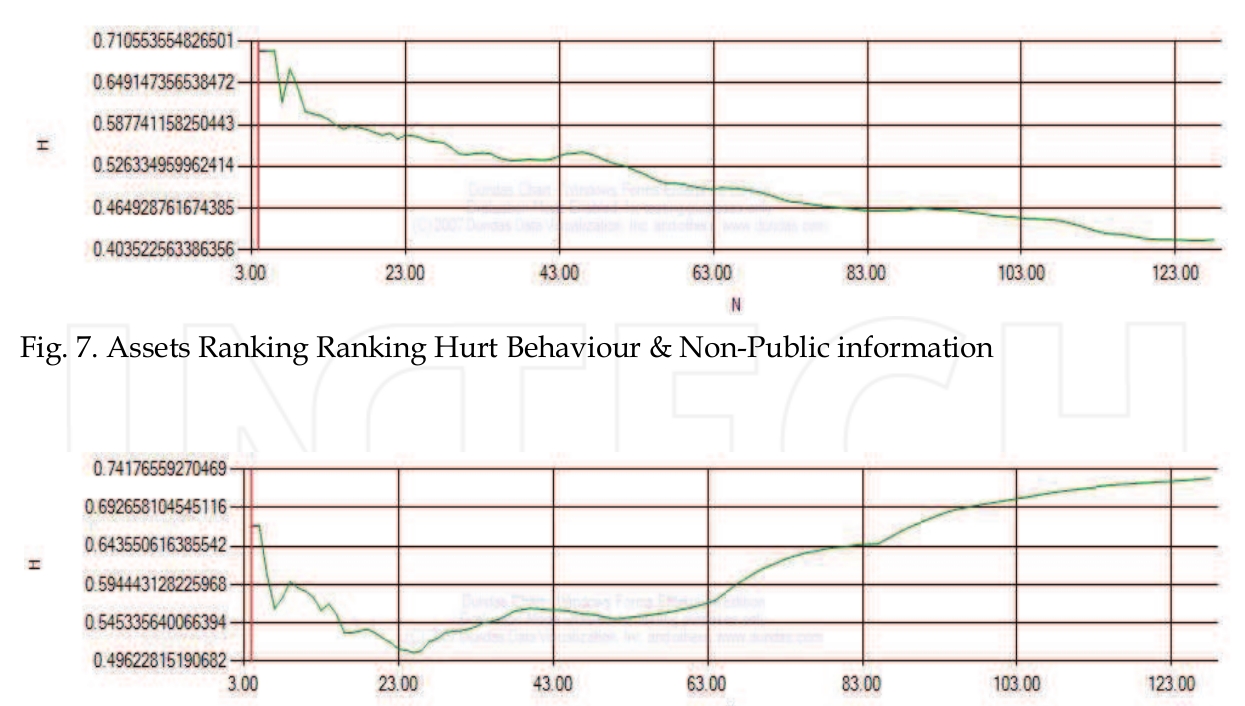
\includegraphics[width=300px]{art1.png}
\end{frame}

\begin{frame}
\frametitle{Análisis dinámico}
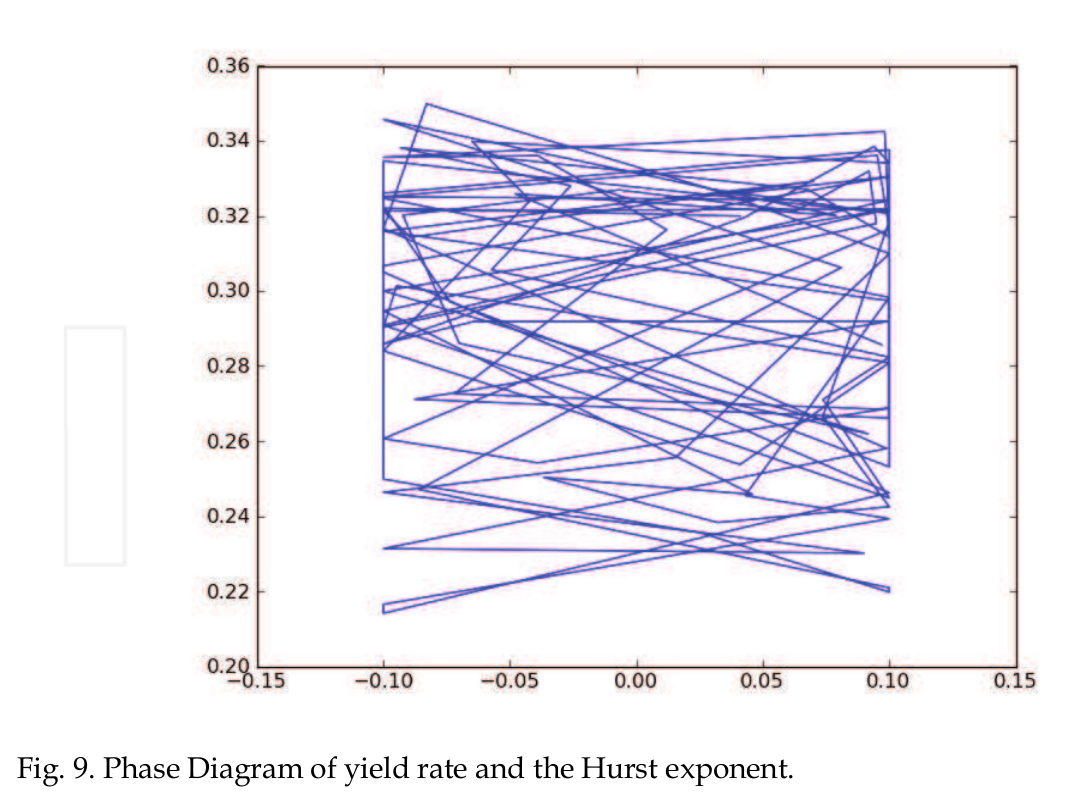
\includegraphics[width=300px]{art2.png}
\end{frame}

\begin{frame}
\frametitle{Conclusiones}

El mercado de capitales es una especie de sistema de auto-retroalimentación. 
muy complejo, y la microestructura formada por el juego la conducta adaptativa de los individuos juega el papel principal. El autómata celular ha proporcionado la posibilidad de describir los factores y sus reglas de interacción. 

Sin embargo, debemos reconocer que el mercado artificial basado en autómatas celulares no está suficiente maduro para construir una nueva teoría de los mercados de capital.

\end{frame}


\end{document}
